\chapter{재규격화, 자연성, 계층성 문제}

\lectureoverview{이 강의의 핵심 발상은 표준 모형의 재규격화에 관한 여러 수수께끼에서 비롯되었다. 따라서 먼저 재규격화의 물리적 의미를 살펴본다. 당면한 문제에 비해 너무 작고 빠른 자유도를 제거하고, 그 효과를 유효한 기술에 담는 것이다. 분자는 그 전형적인 사례다. 이어서 차원 분석을 통해 같은 논리를 스칼라 양자장론에 적용하면, 스칼라 질량의 이차 민감도, 힉스장의 계층성 문제, 페르미온과 게이지 보손이 누리는 보호, 그리고 그보다 훨씬 심각한 진공 에너지 문제를 살펴볼 수 있다.}

\section{문제의 규모에 맞춘 물리학}

이번 분기에 다룰 발상 대부분은 표준 모형의 재규격화에 관한 질문에서 비롯되었다---때로는 수수께끼였고, 때로는 유용한 관찰이었다---. 재규격화에는 두 가지 사고방식이 결합되어 있다. 첫째는 묻고 있는 문제와 무관할 만큼 거리가 짧은 구조를 기술에서 제거하는 것이다. 둘째는 차원 분석으로, 흔히 어려운 적분을 계산하기도 전에 짧은 거리에서의 답을 결정해 준다.

이처럼 세부 사항을 제거하는 일은 물리학 전반에서 일어난다. 원자핵을 이해하고자 할 때 쿼크와 양자 색역학에서 출발할 수 있다. 양성자와 중성자의 질량과 스핀, 그리고 이들의 유효 핵력을 계산하고 나면 여러 목적에서 쿼크 하부 구조를 잊어도 된다. 핵의 운동은 충분히 느리므로 양성자와 중성자의 비상대론적 양자역학이 흔히 더 유용한 기술이 된다.

한 단계 위에서 원자물리학은 보통 원자핵의 내부 구성을 필요로 하지 않는다. 핵물리학은 어떤 원자핵과 동위원소가 존재하는지 알려 주고 질량과 전하 같은 성질을 제공한다. 그런 다음 원자핵과 전자라는 새로운 유효 기본 물체로 다시 시작한다. 쿼크와 양성자, 중성자가 사라진 것은 아니다. 이들의 효과가 원자핵이 지닌 매개변수에 압축되어 들어간 것이다.

어떤 정보를 남길지는 다음 질문에 달려 있다. 원자 계산에는 환산 질량에 들어가는 원자핵의 질량이 필요할 수 있고, 쿨롱장을 결정하는 전하도 반드시 필요하다. 그러나 보통은 어느 쿼크가 원자핵 운동량의 얼마를 갖는지 알 필요가 없다. 원소의 전하 종류는 대략 90가지이며, 동위원소까지 세면 원자핵의 종류는 더 많다. 이 목록은 입력값으로 주어도 된다. 반면 전자는 아직 제거할 수 없다. 전자의 운동이 바로 원자 구조를 이루기 때문이다.

원자 문제를 푼 뒤에는 이와 비슷하게 원자를 분자의 구성 요소로 볼 수 있다. 서스킨드가 익살스럽게 나열한 쿠키 원자, 커피 원자, 초콜릿 원자, 케첩 원자는 각 단계에서 새로운 기술이 시작된다는 진지한 점을 보여 준다. 분자의 성질과 힘을 알고 나면, 매 단계마다 전자 문제를 다시 풀지 않고도 분자를 더 큰 팅커토이 같은 조립체로 결합할 수 있다.

각 단계의 전환은 거친 입자화다. 새 기술은 절대적인 의미에서 덜 정확할 수 있지만, 의도한 규모에서는 훨씬 유용하다. 장에는 임의로 짧은 파장을 포함해 모든 파장의 모드가 있으므로 양자장론에서는 이 문제가 불가피하다. 따라서 분해할 수 없을 만큼 짧은 파장의 효과를 모두 더하고, 이를 새로운 유효 매개변수로 대체한다. 이 과정과 차원 분석이 재규격화의 물리적 내용이다.

\section{분자: 전형적인 사례}

원자 두 개를 놓고 상대 운동을 간단히 기술하는 방법을 생각해 보자. 각 원자는 무거운 원자핵과 전자 구름으로 이루어져 있다. 양성자조차 전자보다 대략 2천 배 무겁고, 더 무거운 원자핵에서는 규모의 차이가 더 커진다. 전자들이 빠르게 움직이며 주위에 흐릿한 구름을 이루는 볼링공 두 개를 떠올리면 유용하다. 원자핵은 느리게 반응하는 반면 전자 상태는 빠르게 재배열된다.

원자핵의 위치와 운동량을 \(R_a\) 및 \(P_a\)라 하고, 두 원자의 질량을 \(M\)라 하자. 전자의 좌표와 운동량은 \(r_i\) 및 \(q_i\)이고, 전자의 질량은 \(m_e\)이다. \(4\pi\epsilon_0\) 같은 통상적인 계수는 생략하면 해밀토니안은 개략적으로 다음과 같다.
\begin{align}
H={}&
\frac{P_1^2}{2M}+\frac{P_2^2}{2M}
+\frac{e^2}{R_{12}}
+\sum_i\frac{q_i^2}{2m_e}
+\frac12\sum_{i\ne j}\frac{e^2}{r_{ij}}
\nonumber\\
&-\sum_i\left(
\frac{e^2}{|R_1-r_i|}
+\frac{e^2}{|R_2-r_i|}
\right).
\label{eq:molecular-hamiltonian}
\end{align}
첫째 줄에는 원자핵의 운동 에너지, 원자핵 사이의 쿨롱 반발력, 전자의 운동 에너지가 들어 있다. 둘째 줄에는 전자 사이의 반발력과 전자-원자핵 인력이 들어 있다. 일반적인 전하를 가진 원자핵의 경우 이에 해당하는 \(Z_a\) 인자를 복원해야 한다. 강의에서는 시간 규모의 분리가 핵심이므로 전하를 개략적으로만 나타낸다.

두 가지 특징적인 운동이 있다. 원자핵은 무겁고 느리며, 전자는 가볍고 빨라 흐릿하게 보일 정도다. 첫 번째 근사에서는 원자핵의 위치를 고정하고 전자에 의존하는 항을 전자 해밀토니안으로 묶는다.
\begin{equation}
H_{\mathrm{el}}(R_1,R_2).
\end{equation}
원자핵의 각 고정된 배치에 대해 다음 고유값 문제를 푼다.
\begin{equation}
H_{\mathrm{el}}(R_1,R_2)
\psi_0(r_1,\ldots,r_N;R_1,R_2)
=
E_{\mathrm{el}}(R_1,R_2)\psi_0.
\label{eq:electronic-ground-state}
\end{equation}
전자 고유값 가운데 가장 낮은 값을 취한다. 전자를 무시한 것이 아니라, 전자의 빠른 운동을 함수 \(E_{\mathrm{el}}(R_1,R_2)\)로 모두 요약한 것이다.

이 논리는 단열적이다. 전자가 빠르게 한 번 조정되는 동안 원자핵은 거의 움직이지 않으므로 좌표를 매개변수로 취급할 수 있다. 전자 고유값 문제를 푼 다음에는 같은 좌표가 다시 움직이도록 둔다. 천천히 변하는 각 배치에서 전자 구름은 순간적인 바닥 상태를 따른다. 더 정확한 처리에서는 들뜬 전자 퍼텐셜 에너지 곡면과 그 사이의 전이를 포함할 수 있지만, 가장 낮은 곡면만으로도 재규격화의 발상이 드러난다.

\begin{figure}[htbp]
\centering
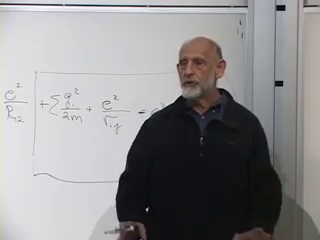
\includegraphics[width=0.72\textwidth]{lecture_01_figure_02.png}
\caption{전자 바닥 상태 문제를 소개하면서 분자의 해밀토니안을 칠판에 남겨 두었다. 이 장면에서 가려진 항들은 식 ~\eqref{eq:molecular-hamiltonian}의 조판된 형태에 나와 있다.}
\lectureframe{00:16:19}
\end{figure}

\begin{classroomqa}
\audiencequestion{원자핵의 운동량을 그냥 0으로 두는 건가요?\lecturetimestamp{00:15:39}}
\lecturerresponse{일시적으로만 그렇다. 첫 번째 근사에서는 원자핵이 전자보다 훨씬 느리게 움직이므로 못으로 고정해 둔 것처럼 취급한다. 유효 원자핵 문제를 풀 때는 운동량을 다시 포함하므로 이 근사는 불확정성 원리를 위배하지 않는다.}
\end{classroomqa}

이제 전자 바닥 상태 에너지는 원자핵이 느끼는 퍼텐셜에 기여한다.
\begin{equation}
V_{\mathrm{eff}}(R_1,R_2)
=\frac{e^2}{R_{12}}+E_{\mathrm{el}}(R_1,R_2).
\label{eq:molecular-effective-potential}
\end{equation}
두 원자만 고립된 경우 회전 및 병진 대칭성에 따라 이 퍼텐셜은 두 원자 사이 거리 \(R_{12}\)의 함수로 줄어든다. 아주 짧은 거리에서는 원자핵의 쿨롱 반발력이 지배적이다. 아주 먼 거리에서는 상호작용이 거의 없다. 그 사이에서는 전자 구름이 인력 영역과 퍼텐셜 에너지의 최솟값을 만들 수 있다. 그러면 원자핵의 파동함수는 그 최솟값 부근에 자리 잡고 결합 분자를 기술한다.

계산의 순서에 주목하자. 경험적으로 인력을 가정한 뒤 전자를 버린 것이 아니다. 먼저 고정된 원자핵 배경에서 전자의 양자 문제를 풀었다. 그런 다음에야 전자의 명시적 좌표를 지우고 그 결과로 얻은 고유값을 남겼다. 짧은 거리 물리학은 \(V_{\mathrm{eff}}\)의 모양과 깊이, 곡률에 그대로 남는다. 최솟값의 위치가 평형 거리를 정하고, 곡률이 작은 진동을 좌우하며, 점근적 형태가 결합 상태의 존재 여부를 결정한다. 하나의 유효 함수가 이 모든 전자 정보를 더 느린 문제로 전달한다.

따라서 복잡한 다전자 해밀토니안은 새로운 퍼텐셜을 갖는 두 핵의 해밀토니안이 되었다. 빠른 자유도는 제거했지만 저에너지에서의 완전한 효과는 남겼다. 퍼텐셜은 재규격화되었다. 익숙한 Born--Oppenheimer 추론은 보통 그런 이름으로 소개되지는 않지만, 우리가 필요로 하는 바로 그 생각을 담고 있다: \begin{equation}
\begin{gathered}
\text{fast microscopic dynamics}\\
\Downarrow\\
\text{effective parameters for slow dynamics}
\end{gathered}
\end{equation}

\section{자연 단위계와 장의 차원}

양자장론에서는 제거할 모드를 짧은 거리, 짧은 파장, 높은 진동수 또는 높은 에너지 모드라고 서로 바꾸어 표현할 수 있다. 그림을 그리기 전에 차원 계산의 기준부터 정하자.

일반 역학에서는 길이, 시간, 질량을 서로 독립적인 단위로 쓴다. 입자물리학에서는
\begin{equation}
\hbar=c=1.
\end{equation}
라고 둔다. 그러면 \(E=mc^2\)에 의해 에너지와 질량이 동등하고, \(c=1\)이므로 길이와 시간이 동등하며, \(\hbar=1\)에 의해 운동량은 길이의 역수가 된다. 남는 차원은 하나뿐이다.
\begin{equation}
[M]=[E]=[p]=L^{-1},
\qquad
[x]=[t]=L.
\label{eq:natural-units}
\end{equation}

차원이 사라지는 것은 아니다. 시간은 길이로, 질량은 길이의 역수로 나타내도록 환산 인자를 정하는 것이다. 한 단위만 정하면 다른 단위는 모두 따라온다. 따라서 절단 에너지는 짧은 거리 \(\delta\)로도, 높은 에너지 \(\Lambda=1/\delta\)로도 나타낼 수 있다. 두 표현은 같은 규모를 서로 다른 언어로 쓴 것이다.

하나의 실수 스칼라장 \(\phi\)를 택하고, 라그랑지언 밀도를 개략적으로 다음과 같이 정규화하자.
\begin{equation}
\mathcal L=(\partial_\mu\phi)(\partial^\mu\phi)-V(\phi),
\qquad
S=\int d^4x\,\mathcal L.
\label{eq:scalar-action}
\end{equation}

\begin{figure}[htbp]
\centering
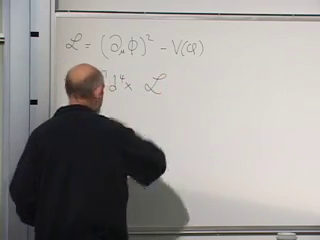
\includegraphics[width=0.78\textwidth]{lecture_01_figure_03.png}
\caption{국소 스칼라 라그랑지언 밀도와 이를 시공간에 적분해 얻는 작용.}
\lectureframe{00:26:08}
\end{figure}

라그랑지언 밀도는 국소적이며, 시공간의 한 점을 기술한다. 작용을 정지시키면 고전적인 장 방정식이 나온다. 양자론에서는 같은 작용이 경로적분의 위상 \(\exp(iS)\)에 들어간다. 어느 관점에서 보더라도 \(S\)의 차원이 중요하다. \(\hbar\)를 복원하면 위상은 \(\exp(iS/\hbar)\)이고, \(\hbar=1\)로 두면 \(S\) 자체가 무차원이어야 한다.

\begin{classroomqa}
\audiencequestion{작용의 단위는 \(\hbar\)인가요?\lecturetimestamp{00:26:13}}
\lecturerresponse{그렇다. \(\hbar\)를 1로 두었으므로 이 단위계에서 작용은 무차원이다. 4차원 측도의 차원은 \(L^4\)이므로 라그랑지언 밀도의 차원은 \(L^{-4}\)이어야 한다.}
\end{classroomqa}

이제 운동항으로 장의 차원이 정해진다.
\begin{align}
[S]&=1, & [\mathcal L]&=L^{-4},\\
[\partial_\mu]&=L^{-1}, &
[(\partial\phi)^2]&=L^{-2}[\phi]^2=L^{-4},\nonumber\\
&& [\phi]&=L^{-1}.
\label{eq:scalar-dimension}
\end{align}
이 간단한 계산으로 뒤에 나올 모든 파인만 도표의 자외선 규모를 정할 수 있다.

퍼텐셜을 다음과 같이 전개하자.
\begin{equation}
V(\phi)=\frac{m^2}{2}\phi^2+g\phi^3+\lambda\phi^4+\cdots.
\label{eq:scalar-potential}
\end{equation}
각 항의 차원은 모두 \(L^{-4}\)이어야 한다. \([\phi^n]=L^{-n}\)이므로,
\begin{equation}
[m^2]=L^{-2},
\qquad
[g]=L^{-1},
\qquad
[\lambda]=1.
\label{eq:coupling-dimensions}
\end{equation}
사차 결합 상수는 무차원이다. 이런 결합 상수는 단순한 길이 거듭제곱만으로는 척도 의존성을 알 수 없기 때문에 재규격화에서 특히 중요하다.

\begin{classroomqa}
\audiencequestion{\(g\)의 단위는 질량인가요?\lecturetimestamp{00:29:52}}
\lecturerresponse{그렇다. 인자 \(\phi^3\)의 차원은 \(L^{-3}\)이고, 퍼텐셜 밀도의 차원은 \(L^{-4}\)이어야 한다. 따라서 \([g]=L^{-1}\)이며, 자연 단위계에서는 질량의 차원이다.}
\end{classroomqa}

\section{꼭짓점과 짧은 거리 전파자}

파인만 규칙은 꼭짓점과 전파자로 이루어진다. 항 \(g\phi^3\)은 세 개의 선이 만나는 꼭짓점을 주며, 여기에 비례하는 인자는 \(g\)이다. 항 \(\lambda\phi^4\)은 네 개의 선이 만나는 꼭짓점을 주며, 여기에 비례하는 인자는 \(\lambda\)이다. 이차항은 국소적인 2점 삽입을 준다. 입자가 들어와 흡수된 뒤 다시 방출되는 것으로 그릴 수 있으며, 계수는 \(m^2/2\)에 비례한다. 강의에서는 단면을 계산하는 대신 척도 의존성을 추출하므로 수치 정규화, 부호, \(i\) 인자와 대칭 인자를 일부러 생략한다.

이 그림들은 실제 과정으로 해석할 수 있다. 3점 꼭짓점은 양자 두 개를 흡수하고 하나를 방출하는 과정일 수도 있고, 세 선을 교차 대칭에 따라 다르게 배정한 과정일 수도 있다. 4점 꼭짓점은 입자 두 개가 들어와 두 개가 나가는 과정을 기술할 수 있다. 이차 교차 표시는 보통 자유 전파자에 포함되지만, 여전히 가능한 2선 꼭짓점이다. 잠시 후 분해되지 않은 모든 2점 과정은 이것과 비교해 알아볼 수 있으므로 여기서 표시해 둔다.

전파자는 시공간의 두 점을 연결한다. 전파자 선은 양자 입자가 고전적인 직선 경로를 따라 움직였다는 뜻이 아니다. 이는 \(x\)에서 장 여기 상태를 만들고 \(y\)에서 제거하거나 검출할 진폭을 나타낸다.
\begin{equation}
\Delta(x-y)=\langle0|\phi(y)\phi(x)|0\rangle.
\label{eq:position-propagator}
\end{equation}
식을 오른쪽에서부터 읽어 보자. 진공에 \(\phi(x)\)를 작용시키면 \(x\)에 한 입자 성분이 생성된다. 브라에 \(\phi(y)\)를 작용시키면 \(y\)에서 그 성분이 제거된다. 두 작용의 진공 행렬원소는 첫 번째 점에서 생성된 상태와 두 번째 점에서 검출된 상태 사이의 중첩 진폭이다. 기호 \(x\)와 \(y\)는 두 개의 카르테시안 좌표만이 아니라 4차원 벡터 전체를 가리킨다.

상태에는 물리적 차원이 없고 장마다 \(L^{-1}\)가 기여한다. 따라서
\begin{equation}
[\Delta]=L^{-2}.
\end{equation}
질량 없는 장에는 고유한 길이 척도가 없으므로 차원 분석에 따라 짧은 거리에서의 거동은 다음과 같다.
\begin{equation}
\Delta(x-y)\sim\frac{1}{(x-y)^2}.
\label{eq:massless-propagator}
\end{equation}
분모는 로런츠 불변인 거리 제곱이며, 특이점에서는 통상적인 처방이 필요하다.\editorialnote{승수 계산에는 유클리드 거리로 위크 회전하면 편리하다. 이때 크기는 모호함 없이 \(1/|x-y|^2\)에 비례한다. 이 변환은 아래에서 사용하는 자외선 거듭제곱을 바꾸지 않는다.}

\(y\)가 \(x\)에 가까워지면 전파자는 발산한다. 분리 거리가 사라질 때 나타나는 전파의 특이성이 더 복잡한 도표에서 자외선 발산이 생겨나는 근원이다.

\section{스칼라 질량의 재규격화}

스칼라장의 동역학적 매개변수는 \(m^2\)이다. 이는 상대론적 분산 관계만 보아도 알 수 있다.
\begin{equation}
E=\sqrt{\mathbf p^2+m^2}.
\end{equation}
유효 기술이 분해하는 가장 짧은 거리를 \(\delta\)라 하자. 꼭짓점 사이 거리가 \(\delta\)보다 짧은 과정은 구별하지 않기로 한다. 들어오는 스칼라 하나와 나가는 스칼라 하나가 있는, 분해되지 않은 과정은 관측 가능한 형태가 질량 삽입과 같으므로 유효 질량에 기여해야 한다.

가속기를 현미경이라고 생각해 보자. 가장 정밀한 분해능이 \(\delta\)라면, 한 점에서 입자가 흡수된 다음 \(\delta\)보다 훨씬 짧은 거리 뒤에서 방출되는 과정은 진정한 국소 사건과 구별할 수 없다. 그 길이 규모의 꼭짓점들을 의도적으로 흐릿하게 본다. 재규격화란 분해능 아래의 모든 대안을 해당 국소 연산자의 계수에 반영하는 규칙이다.

\subsection{첫 번째 사차 보정}

\(\phi^4\) 꼭짓점 하나에서 시작하자. 두 다리는 외부 입자이고, 나머지 두 다리는 거의 같은 지점에서 방출되었다가 재흡수되는 짧은 고리를 이룬다. 일치하는 점의 전파자를 절단 거리만큼 퍼뜨리면
\begin{equation}
\Delta(0)\ \longrightarrow\ \Delta(\delta)\sim\frac{1}{\delta^2},
\end{equation}
따라서
\begin{equation}
\delta m^2_{(1)}\sim\frac{\lambda}{\delta^2}.
\label{eq:one-loop-scalar-mass}
\end{equation}
\(m_0^2\)가 입력값 또는 맨 처음의 매개변수라면, 낮은 분해능에서의 2점 계수는 개략적으로 다음과 같다.
\begin{equation}
\frac{m_{\mathrm{eff}}^2}{2}
\sim
\frac{m_0^2}{2}
+c_1\frac{\lambda}{\delta^2},
\label{eq:first-renormalized-mass}
\end{equation}
여기서 \(c_1\)에는 무시한 수치 인자와 관례에 따라 달라지는 인자가 들어 있다. \(\delta\)보다 짧은 거리를 분해하지 못하는 실험에서 측정하는 실험실 질량은 \(m_0\) 자체가 아니라 이렇게 재규격화된 양이다.

따라서 관측된 2점 사건이 일어나는 방식은 서로 구별할 수 없는 두 가지다. 원래의 이차 꼭짓점에서 입자가 흡수되었다가 재방출될 수도 있고, 사차 상호작용에서 가상 스칼라를 잠시 방출했다가 재흡수하는 방식으로 같은 일이 일어날 수도 있다. 양자역학에서는 진폭을 더한다. 고리가 분해능보다 작은 영역에 놓이면 그 개별 과정은 유효 기술에서 사라지지만, 측정되는 계수에 대한 기여는 남는다.

\subsection{다음 사차 보정}

이번에는 사차 꼭짓점 두 개를 연결하자. 외부 입자 하나가 \(x\)에서 들어오고 하나가 \(x+\Delta\)에서 나가며, 세 개의 내부 전파자가 두 꼭짓점을 잇는다. \(\lambda\)은 두 번 곱해지고, 전파자들은 \(\Delta^{-6}\)를 준다. 양자 진폭은 나가는 입자가 나타날 수 있는 분해되지 않은 모든 위치에 대해 더해야 하므로, 상대 4차원 벡터를 적분한다.
\begin{equation}
\delta m^2_{(2)}
\sim
\lambda^2
\int_{|\Delta|\gtrsim\delta}
d^4\Delta\,\frac{1}{|\Delta|^6}.
\label{eq:two-loop-power-count}
\end{equation}

\begin{classroomqa}
\audiencequestion{꼭짓점의 작은 표시를 보면 입자가 세 개만 있다는 뜻인가요?\lecturetimestamp{00:46:35}}
\lecturerresponse{아니다. 여전히 사차 상호작용을 사용한다. 각 꼭짓점에는 네 개의 선이 만나며, 이 2점 도표에서는 한 선이 외부선이고 세 선이 두 꼭짓점 사이를 지난다. 두 번째 꼭짓점에도 네 개의 선이 들어온다.}
\end{classroomqa}

측도는 길이의 4제곱을 주고 세 전파자는 길이의 -6제곱을 준다. 이 계산에서 유일한 척도는 자외선 절단이므로,
\begin{equation}
\int_{|\Delta|\gtrsim\delta}
\frac{d^4\Delta}{|\Delta|^6}
\sim\frac{1}{\delta^2},
\qquad
\delta m^2_{(2)}
\sim\frac{\lambda^2}{\delta^2}.
\label{eq:two-loop-scalar-mass}
\end{equation}
여기서 \(\Delta^\mu\)는 네 성분을 가진 적분 변수다. 시간 성분과 공간 성분 세 개에 대해 적분한다. 소문자 \(\delta\)는 고정된 절단 길이다. 강의에서는 처음에 두 기호를 같은 이름으로 부르다가 뒤에 표기를 바로잡는다.

4차원 측도를 반지름 방향으로 적으면 같은 결과를 확인할 수 있다. 각도에 따른 상수 인자를 제외하면
\begin{equation}
\int_{\delta}\frac{d^4\Delta}{|\Delta|^6}
\sim
\int_{\delta}\frac{R^3\,dR}{R^6}
=\int_{\delta}\frac{dR}{R^3}
\sim\frac{1}{\delta^2}.
\end{equation}
이것이 자외선 추정에서 큰 거리 쪽 적분 상한이 중요하지 않은 이유다. 적분값은 하한에서 주로 결정된다.

더 높은 차수의 도표에서도 같은 양상이 반복된다. 사차 꼭짓점이 더 많은 도표에서는 \(\lambda\)의 거듭제곱이 더 높아지지만, 차원 분석에 따르면 여전히 질량에 이차 발산 기여가 가능하다.
\begin{equation}
\begin{aligned}
m_{\mathrm{eff}}^2
={}&m_0^2
+\frac{1}{\delta^2}
\left(c_1\lambda+c_2\lambda^2+c_3\lambda^3+\cdots\right)\\
&+\text{weaker terms}.
\end{aligned}
\label{eq:scalar-mass-series}
\end{equation}

\subsection{삼차 상호작용과 로그}

삼차 꼭짓점 두 개 사이에는 가까운 두 점을 잇는 전파자 두 개가 있다. 이들의 기여는 다음과 같이 스케일링한다.
\begin{equation}
\delta m_g^2
\sim
g^2\int_{|\Delta|\gtrsim\delta}
\frac{d^4\Delta}{|\Delta|^4}.
\label{eq:cubic-loop}
\end{equation}
이제 측도와 분모의 거듭제곱이 같다. 남는 의존성은 거듭제곱이 아니라 로그다.
\begin{equation}
\delta m_g^2
\sim
c_g g^2\log\!\left(\frac{1}{\mu\delta}\right).
\label{eq:cubic-log}
\end{equation}
기준 척도 \(\mu\)를 넣으면 로그의 인자가 무차원이 된다. 이것이 강의의 개략적인 \(g^2\log\delta\)을 차원을 갖춘 형태로 나타낸 것이다. 로그는 역수 거듭제곱보다 훨씬 느리게 변하므로 절단 길이가 짧아질수록 \(1/\delta^2\)이 지배적이다.

이번에도 반지름 방향으로 쓰면 차이가 분명해진다.
\begin{equation}
\int_{\delta}^{R_{\mathrm{IR}}}
\frac{d^4\Delta}{|\Delta|^4}
\sim
\int_{\delta}^{R_{\mathrm{IR}}}\frac{R^3\,dR}{R^4}
=\log\!\left(\frac{R_{\mathrm{IR}}}{\delta}\right).
\end{equation}
측도와 분모의 거듭제곱이 같으면 로그가 생긴다. 분모의 거듭제곱이 더 크면 절단 길이의 역수 거듭제곱이 생긴다. 강의의 목적은 각도 인자를 계산하는 것이 아니라, 자외선에서의 답을 한눈에 알아보는 것이다.

\begin{classroomqa}
\audiencequestion{로그의 밑은 무엇인가요?\lecturetimestamp{00:57:42}}
\lecturerresponse{자연로그를 쓴다. 밑을 바꾸면 로그에 수치 상수만 곱해지며, 그 상수는 여기서 계산하지 않은 \(2\), \(\pi\), 대칭 인자들을 포함하는 계수에 흡수된다.}
\end{classroomqa}

\begin{classroomqa}
\audiencequestion{길이의 로그를 어떻게 취할 수 있나요? 질량 보정항의 단위는 어디서 나오나요?\lecturetimestamp{00:58:32}}
\lecturerresponse{로그는 언제나 두 척도를 비교한다. 따라서 실제로는 \(1/(\mu\delta)\) 같은 무차원 비의 로그를 취하는 것이다. 결합 상수 \(g\)는 질량의 차원을 한 번 가지므로, \(g^2\)는 보정항에 필요한 질량 제곱 차원을 이미 정확히 갖는다.}
\end{classroomqa}

\begin{classroomqa}
\audiencequestion{파인만 도표는 진폭을 준다고 하셨는데, 그 절댓값의 제곱이 확률인가요?\lecturetimestamp{00:59:41}}
\lecturerresponse{필요한 상태 인자와 위상 공간 인자를 포함해 물리적 전이 계산에 넣으면 그렇다. 여기서 진폭의 더 직접적인 역할은 다르다. 분해되지 않은 2점 진폭은 질량항과 같은 국소 형태이므로 유효 질량 매개변수를 이동시킨다.}
\end{classroomqa}

\section{모든 매개변수는 유효량이 된다}

질량 도표가 무한히 많다는 사실은 \(\lambda\)가 작다고 해서 사라지지 않는다. 섭동론에서는 이들을 결합 상수의 거듭제곱에 따라 순서 짓기 때문에 연속되는 항이 차례로 작아질 수 있지만, 항의 수는 여전히 무한하다. 같은 짧은 거리 자유도 제거 과정은 상호작용 자체도 재규격화한다.

\begin{classroomqa}
\audiencequestion{질량 재규격화에도 도표가 무한히 많지 않나요?\lecturetimestamp{01:00:35}}
\lecturerresponse{그렇다. \(\lambda\)가 충분히 작으면 더 높은 거듭제곱의 항이 차례로 억제되므로 섭동 급수가 유용할 수 있다. 그래도 재규격화된 매개변수는 첫 번째 그림 하나가 아니라 급수 전체로 정의된다.}
\end{classroomqa}

실제로 국소적인 \(\lambda\phi^4\) 상호작용은 입자 두 개가 들어오고 두 개가 나가는 진폭이다. 더 복잡한 4점 과정이 분해되지 않은 영역 안에서 모두 일어나면 낮은 분해능에서는 원래의 국소 꼭짓점과 구별할 수 없다. 따라서 그런 도표의 기여를 유효한 \(\lambda\)에 합쳐 넣는다. 4차원 \(\phi^4\) 이론에서 그 주된 척도 의존성은 보통 로그 형태다. 강의에서는 베타 함수를 계산하지 않고 이 사례로 일반적인 점을 설명한다.
\begin{equation}
\begin{gathered}
\text{parameters measured at low energy}\\
\ne\\
\text{parameters entered at the microscopic cutoff}
\end{gathered}
\end{equation}

4점 사례가 중요한 이유는 재규격화가 질량 발산에만 적용하는 특별한 보수 작업이라는 오해를 없애기 때문이다. 라그랑지언에서 허용되는 모든 연산자는 같은 외부선을 갖고 같은 대칭성을 따르는 분해되지 않은 도표로 재현될 수 있다. 2점 과정은 이차 계수를, 4점 과정은 사차 계수를 재규격화하며, 진공에서 진공으로 가는 과정은 상수항을 재규격화한다. 저에너지 라그랑지언은 이런 짧은 거리 과정 모두를 기록하는 간결한 장부다.

\begin{classroomqa}
\audiencequestion{\(\Delta\)의 단위가 길이라면 그 로그는 차원상 이상하지 않나요? 칠판에서는 대문자 델타와 소문자 델타를 바꿔 쓴 건가요?\lecturetimestamp{01:01:34}}
\lecturerresponse{로그는 실제로 다른 척도에 대한 비를 뜻하므로 무차원이다. 맞다. 표기를 잠시 뒤바꾸어 썼다. \(\Delta^\mu\)는 적분 변수이고, \(\delta\)는 최종 답에 남는 하한 거리 절단이다.}
\end{classroomqa}

이것은 분자 사례에 대응하는 장론의 설명이다. 보이지 않는 빠른 전자를 풀고 그 결과를 퍼텐셜에 넣었다. 여기서는 보이지 않는 짧은 거리 과정을 모두 더하고 그 결과를 질량과 결합 상수, 그리고 허용되는 모든 국소 계수에 넣는다. 모든 항이 이동한다.

\begin{classroomqa}
\audiencequestion{실험에서 볼 수 없는 척도보다 짧은 척도까지 측정된 양에 포함되는지 다시 말씀해 주시겠어요?\lecturetimestamp{01:05:13}}
\lecturerresponse{그렇다. 개별 요동은 분해되지 않지만, 그 효과를 모두 더한 결과는 포함된다. 더 짧은 척도와 관련된 모든 도표의 기여를 하나의 유효 계수에 모으며, 저에너지 실험에서는 이를 예컨대 물리적 질량 제곱이라고 부른다.}
\end{classroomqa}

\begin{classroomqa}
\audiencequestion{그렇다면 입력항 \(m_0^2\)이 나머지 기여를 상쇄해야 하나요?\lecturetimestamp{01:06:00}}
\lecturerresponse{측정된 스칼라 질량이 개별 자외선 기여보다 훨씬 작다면 그렇다. 필요한 상쇄가 바로 이제 살펴볼 미세 조정 문제다.}
\end{classroomqa}

\section{힉스 계층성 문제}

절단 길이가 플랑크 길이라고 가정하자. 그러면 유효장론은 실험실 규모에서 양자 중력이 개입해야 하는 규모까지의 요동을 모두 요약해야 한다. 입자물리학 단위로는
\begin{equation}
\delta\sim M_{\mathrm{Pl}}^{-1}\sim10^{-19}\,\mathrm{GeV}^{-1},
\qquad
\frac{1}{\delta^2}\sim10^{38}\,\mathrm{GeV}^2.
\label{eq:planck-cutoff}
\end{equation}
환산 플랑크 척도를 쓰든 환산하지 않은 플랑크 척도를 쓰든, 엄청난 차이를 비교한다는 점은 달라지지 않는다.

플랑크 길이는 양성자 반지름보다 약 열아홉 자릿수 작고, 논의 중인 가속기들이 직접 탐사하는 거리보다 대략 열여섯에서 열일곱 자릿수 작다. 이 길이 차이를 제곱하면 길이의 큰 계층 구조가 스칼라 질량제곱 매개변수에서 대략 서른네 자릿수 규모의 상쇄로 이어진다.

스칼라인 힉스장의 바람직한 약한 상호작용 척도는 수백 GeV 정도이지, \(10^{19}\) GeV가 아니다. 그런데 식 ~\eqref{eq:scalar-mass-series}의 항들은 자연스럽게 플랑크 척도 크기가 될 수 있다. 각 항의 부호는 따져 보지 않았다. 양수인 항도 음수인 항도 있을 수 있고, 맨 처음의 질량 제곱도 어느 부호든 가질 수 있다. 그러나 전기약 척도의 나머지 값을 남기려면 이처럼 거대한 항들이 대략 소수점 아래 34자리까지 상쇄되어야 한다. 서스킨드는 처음에 17자리라고 했다가 비교 대상이 질량의 제곱임을 감안해 바로잡는다. 이 조정의 정도를 나타내는 것은 제곱한 비다.

\begin{classroomqa}
\audiencequestion{\(\lambda\)는 1보다 작습니까, 큽니까?\lecturetimestamp{01:09:50}}
\lecturerresponse{1보다 약간 작은 값으로 가정합니다. 연속되는 차수의 항이 커진다면 섭동 이론은 다루기 어려워지고, 순수 스칼라 이론도 사중 결합이 임의로 커지는 경우 일관되게 외삽할 수 없습니다. 하지만 \(\lambda\)는 \(10^{-38}\)만큼 작지는 않습니다. 이 강의에서는 감을 잡기 위해 퍼센트 규모의 값을 사용합니다.}
\end{classroomqa}

\begin{classroomqa}
\audiencequestion{\(\lambda<1\)라고 해도, 각 항에 큰 컷오프 인자가 곱해지므로 중요한 항이 많이 남지 않습니까?\lecturetimestamp{01:10:43}}
\lecturerresponse{그렇습니다. 고차 항들은 결국 급수를 억제하지만, 그렇게 되기 전까지 많은 항이 기여할 수 있습니다. 그 항들과 맨 처음 항이 모두 서로 맞물려 상쇄되어야만 물리적으로 관측되는 값이 그토록 작아집니다.}
\end{classroomqa}

힉스 질량 매개변수가 약한 규모라는 사실을 어떻게 아는지 되짚어 봅시다. 이 강의의 표기법에 따라 대칭 깨짐 퍼텐셜을 다음과 같이 씁니다.
\begin{equation}
V(\phi)=-\frac{\mu^2}{2}\phi^2+\frac{\lambda}{4}\phi^4.
\label{eq:higgs-potential}
\end{equation}
음의 이차항 계수 때문에 원점은 불안정하고, 양의 사차항은 퍼텐셜을 안정화합니다. 미분하면
\begin{equation}
\frac{dV}{d\phi}=-\mu^2\phi+\lambda\phi^3
=\phi(-\mu^2+\lambda\phi^2),
\end{equation}
영이 아닌 극솟값을 얻습니다.
\begin{equation}
\phi_{\min}^2=f^2=\frac{\mu^2}{\lambda}.
\label{eq:higgs-minimum}
\end{equation}
판서에서는 사차항을 \(\lambda\phi^4\)처럼 개략적으로 쓰지만, ~\eqref{eq:higgs-minimum}을 인용합니다. 관례적인 인자 \(1/4\)를 넣으면 논지를 바꾸지 않고도 두 식이 서로 일치합니다.

\(-\mu^2\)의 부호는 중요하지만 자연성 문제를 해결해 주지는 않습니다. 자발적 대칭 깨짐을 일으키는 것은 원점에서의 음의 곡률입니다. 재규격화는 그 곡률을 큰 양의 항과 음의 항만큼 이동시킵니다. 관측된 깨진 진공을 얻으려면 두 항의 합이 단지 작기만 해서는 안 됩니다. 극솟값이 약한 규모에 놓이도록 특정한 작은 음수여야 합니다.

\(W\) 보손과 \(Z\) 보손의 질량으로부터, 이 강의에서 사용하는 대략적인 정규화에서는 \(f\)가 \(200\,\mathrm{GeV}\) 규모임을 알 수 있습니다. \(\lambda\)가 엄청나게 크지도 터무니없이 작지도 않다면, \(\mu\)도 대체로 비슷한 규모여야 합니다. 따라서 관측된 약한 규모의 계수는 각각 수십 자릿수 더 클 수도 있는 기여들의 잔여분입니다.

이를 힉스 미세 조정 문제, 계층 문제 또는 게이지 계층 문제라고 합니다. 여기서 계층이란 보통의 약한 규모와 가능한 대통일 규모 또는 플랑크 규모 사이의 엄청난 비율을 뜻합니다. 작은 수라는 사실만으로 반드시 역설이 되는 것은 아닙니다. 여기서 문제를 일으키는 것은 크고 서로 무관해 보이는 항들을 극도로 정밀하게 상쇄해 만들어 낸 작은 수입니다. 이 문제는 1970년대 후반과 1980년대 초반에 인식되었으며, 그 상쇄의 배후에 있는 메커니즘을 찾으려는 노력이 초대칭과 여러 경쟁 이론의 동기가 됩니다.

무한한 섭동 급수는 이 수수께끼를 없애기보다 더 두드러지게 합니다. 퍼센트 규모의 \(\lambda\)라면 충분히 고차인 거듭제곱은 작아지지만, 억제가 우세해지기 전에 많은 항이 나타날 수 있습니다. 한 루프가 우연히 맨 처음 질량을 상쇄하는 것만으로는 충분하지 않습니다. 나머지 단거리 과정까지 포함한 뒤에도 유효한 약한 규모가 안정적으로 유지되어야 합니다. 항들 사이의 구조적 관계가 있다면 설명이 되겠지만, 서로 무관한 숫자들을 자릿수마다 맞춰 상쇄하는 것은 미세 조정일 뿐입니다.

\section{페르미온 질량은 왜 더 잘 다루어지는가}

표준 모형의 다른 입자들은 같은 종류의 독립적인 미세 조정을 필요로 하지 않습니다. 디랙 페르미온의 질량항은 다음과 같습니다.
\begin{equation}
\mathcal L_m=-m\bar\psi\psi
=-m\left(\bar\psi_L\psi_R+\bar\psi_R\psi_L\right).
\label{eq:fermion-mass}
\end{equation}
여기에는 질량의 제곱이 아니라 질량이 들어가며, 왼손성과 오른손성을 결합합니다. 따라서 국소적인 질량 삽입은 \(L\)를 \(R\)로, 또는 \(R\)을 \(L\)로 바꿉니다.

\begin{figure}[htbp]
\centering
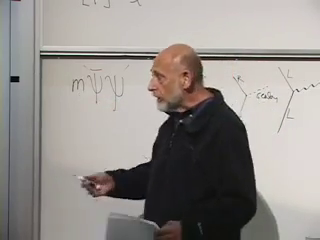
\includegraphics[width=0.76\textwidth]{lecture_01_figure_04.png}
\caption{페르미온 질량항과 손지기성을 바꾸는 선 도식. 분필로 그린 내용 일부가 가려져 있어, 아래에서는 대수적으로 도식을 재구성합니다.}
\lectureframe{01:23:36}
\end{figure}

강의 중에는 흔히 손잡이성 또는 헬리시티라는 말을 씁니다. 정확한 보호를 가장 명확히 나타내려면 손지기성으로 설명하는 것이 좋습니다. 초상대론적 입자의 경우 헬리시티 그림이 의도한 직관을 제공하지만, ~\eqref{eq:fermion-mass}에서 왼손 및 오른손 장이 지니는 양은 손지기성입니다.

게이지 상호작용은 손지기성을 보존합니다.
\begin{equation}
L\xrightarrow{\ \gamma\ }L,
\qquad
R\xrightarrow{\ \gamma\ }R.
\label{eq:gauge-preserves-chirality}
\end{equation}
스칼라와의 유카와 상호작용은 반대 손지기성을 연결합니다.
\begin{equation}
L\xleftrightarrow{\ \phi\ }R.
\label{eq:scalar-flips-chirality}
\end{equation}
먼저 전자가 \(m_0=0\)에서 시작한다고 합시다. 광자를 몇 개나 방출하고 재흡수하더라도 질량이 생길 수는 없습니다. 모든 게이지 꼭짓점이 손지기성을 보존하기 때문입니다. 왼쪽에서 시작한 상태는 계속 왼쪽으로 남습니다. 따라서 순수 양자전기역학에서는 질량이 없는 전자를 일관되게 허용합니다. 전자기 자기 에너지는 질량이 0인 상태에서 가산적인 질량을 만들어 낼 수 없습니다.

선 도식으로 보면 왼손 손지기 전자에서 시작합니다. 첫 번째 광자 꼭짓점에서도 왼손 손지기 상태이며, 전파된 뒤 광자를 재흡수하고 나서도 여전히 왼손 손지기 상태입니다. 이 과정을 반복하면 손지기성을 보존하는 꼭짓점만 더 삽입됩니다. 외부 두 점 함수는 재규격화될 수 있지만, 질량을 정의하는 왼손과 오른손의 구조를 얻을 수는 없습니다.

스칼라 방출은 어떨까요? 스칼라 꼭짓점 하나는 \(L\)를 \(R\)로 바꾸지만, 방출된 스칼라는 다시 흡수되어야 합니다. 따라서 두 점 자기 에너지 도식에는 스칼라 꼭짓점이 짝수 개 들어갑니다. 두 번째 뒤집힘은 첫 번째를 되돌리므로, 전체 도식은 다시 외부 손지기성을 보존합니다. 내부 도식이 아무리 복잡해져도 스칼라의 방출과 재흡수는 꼭짓점들을 짝지어, 처음 질량이 0일 때 가산적인 \(L\)에서 \(R\)로의 항이 나타나지 못하게 합니다.

이는 뒤집힘 횟수의 홀짝성에 관한 논증입니다. 스칼라 꼭짓점 하나는 손지기성을 한 번 뒤집습니다. 내부 스칼라 선을 모두 닫으려면 두 번째 끝점, 곧 두 번째 뒤집힘이 필요합니다. 스칼라 꼭짓점이 네 개면 네 번 뒤집히는 식입니다. 짝수 번 뒤집히면 페르미온은 원래 손지기성으로 돌아옵니다. 이 결론은 판서에 그린 가장 단순한 루프에만 국한되지 않습니다.

도식에 질량 삽입이 이미 포함되어 있어야 비영 질량 보정이 가능해집니다. 예를 들어, 광자의 방출과 재흡수 사이에 \(m_0\bar\psi\psi\) 삽입 하나가 놓일 수 있습니다. 게이지 꼭짓점은 전하의 제곱에 해당하는 인자를 두 개 제공하지만, 손지기성을 뒤집는 유일한 과정은 처음 질량을 제공합니다.
\begin{equation}
\begin{aligned}
m_e
&=m_0+c_1e^2m_0+c_2e^4m_0+\cdots\\
&=m_0\left(1+c_1e^2+c_2e^4+\cdots\right).
\end{aligned}
\label{eq:multiplicative-fermion-mass}
\end{equation}
\(m_0=0\)이면 결과는 계속 0입니다. \(m_0\)가 작으면 모든 보정이 그 작은 값에 비례합니다. 전자가 근본적인 규모에 비해 왜 가벼운지는 여전히 물을 수 있지만, 그 질량을 얻기 위해 서로 무관한 거대한 수들을 빼고 있지는 않습니다. 이런 의미에서 작은 페르미온 질량은 기술적으로 자연스럽습니다.

질량 삽입으로 허용되는 순서가 명확해진다. \(L\)에서 시작하자. 광자 방출은 \(L\)을 보존하고, 삽입된 \(m_0\)는 \(L\)을 \(R\)로 바꾼다. 광자의 재흡수는 \(R\)를 보존한다. 이제 이 다이어그램은 질량항과 같은 외부 키랄리티를 갖지만, 그 값에는 반드시 \(m_0\) 인자가 포함된다. 이것이 ~\eqref{eq:one-loop-scalar-mass}과 결정적으로 다른 점이다. 그 식의 스칼라 보정은 처음의 스칼라 질량을 영으로 두더라도 0이 되지 않는다.

게이지 보손에도 비슷한 보호가 있습니다. 게이지 대칭은 독립적인 질량항을 금지하므로, 질량이 없는 상태에서 시작한 게이지 보손은 모든 섭동 차수에서 질량이 없습니다. 표준 모형에서는 힉스 기대값에 따라 페르미온과 약한 게이지 보손의 질량이 생깁니다. 힉스 규모를 제어하면, 나머지 가벼운 질량에 같은 파국적 미세 조정을 각각 별도로 적용할 필요가 없습니다.

이로써 초대칭이 다루려는 문제가 드러납니다. 이론이 힉스 스칼라에 거대한 가산적 질량 보정이 생기는 것을 막을 수 있을까요? 적절한 초대칭 이론에서는 그렇습니다. 보손 기여와 페르미온 기여가 서로 독립적이지 않고 관계를 맺기 때문입니다. 구체적인 메커니즘은 다음 강의에서 다룹니다.

\section{또 다른 미세 조정 문제: 진공 에너지}

훨씬 더 심각한 재규격화 문제가 하나 있지만, 중력이 포함되어야 관측할 수 있습니다. 중력이 없는 물리에서는 모든 에너지에 상수를 더해도 어떤 실험 결과도 달라지지 않습니다. 예를 들어 전자 질량은 절대적인 에너지가 아닙니다. 진공에 전자 하나를 더하는 데 필요한 추가 에너지입니다.
\begin{equation}
m_e=E(\text{vacuum}+\text{one electron})-E(\text{vacuum})
\end{equation}
이는 전자의 정지 계에서 그렇습니다. 진공과 모든 들뜬 상태가 함께 이동한다면, 그 차이는 변하지 않습니다.

그럼에도 진공에서 진공으로 이어지는 도식은 진공 에너지를 이동시킵니다. \(\lambda\phi^4\) 이론에서는 사차 꼭짓점 하나의 네 다리를 두 개의 짧은 루프로 연결할 수 있습니다. 한 점에서의 전파인자마다 \(1/\delta^2\)가 주어지므로,
\begin{equation}
\delta\rho_{\mathrm{vac}}
\sim
c_{\mathrm{vac}}\frac{\lambda}{\delta^4}.
\label{eq:vacuum-energy-divergence}
\end{equation}
더 복잡한 진공 도식에는 서로 다른 결합상수와 계수가 들어가지만, 차원 분석을 하면 에너지 밀도는 대체로 같은 사차 컷오프 민감도를 갖습니다.

외부 선이 없다는 점이 바로 이 보정을 식별하는 특징입니다. 두 점 도식은 한 입자 상태와 진공을 비교해 질량을 바꾸고, 네 점 도식은 산란을 바꾸며, 들어오거나 나가는 입자가 없는 도식은 진공에서 진공으로의 진폭 자체를 바꿉니다. 사차 꼭짓점 하나가 \(\lambda\)를 제공하고, 짧은 루프 두 개가 각각 \(\delta^{-2}\)를 제공합니다. 따라서 차원 분석에 따르면 에너지 밀도 규모는 \(\delta^{-4}\)여야 합니다.

중력이 없다면 에너지의 가산 상수를 선택해도 되므로 누가 신경 쓰겠느냐고 물을 수 있습니다. 일반 상대성 이론에서는 그 자유가 사라집니다. 에너지-운동량이 시공간 곡률의 원천이므로, 균일한 진공 에너지도 빈 공간을 중력에 반응하게 만듭니다. 진공 에너지는 우주 상수로 나타나며 관측상 암흑 에너지와 연결됩니다. 따라서 측정된 진공 에너지가 작으려면 \(\delta^{-4}\) 형태의 기여들을 상쇄한 뒤에도 그 값이 작게 남아야 합니다.

중력을 켜면 질문이 달라지는 이유가 여기에 있습니다. 보통의 양자역학에서는 모든 에너지 준위를 같은 상수만큼 이동해도 전이 진동수는 바뀌지 않습니다. 중력에서는 그 상수가 아무런 영향을 주지 않는 항이 아닙니다. 진공 응력 텐서는 계량 텐서에 비례해 시공간을 휘게 합니다. 임의로 정할 수 있었던 에너지의 영점이 아인슈타인 방정식의 원천이 됩니다.

따라서 자연성에 관한 심각한 수수께끼는 적어도 두 가지입니다. 강의에서는 진공 에너지 미세 조정에 대략 123자리, 힉스 질량 미세 조정에 대략 30--35자리가 필요하다고 합니다. 정확한 자릿수는 자외선 규모와 관례에 따라 달라지지만, 둘 사이의 차이는 분명합니다. 초대칭은 여기서 논의한 힉스 문제에 대한 가능한 대응입니다. 초대칭이 깨지고 나면, 그것만으로 관측된 우주 상수를 설명하지는 못합니다.\editorialnote{이것은 보손--페르미온의 정확한 초대칭 상쇄가 관측된 진공 에너지에 대한 현상론적 해법이 될 수 없는 이유이기도 합니다. 우리 세계에서는 초대칭이 깨져야 합니다.}

\section{강의 마무리 질의응답}

\begin{classroomqa}
\audiencequestion{\(\delta\)에 따라 힉스 보정이 달라지지만, 컷오프는 임의적으로 보입니다. 플랑크 길이일 수도 있고, 플랑크 길이의 열 배일 수도 있고, 다른 값일 수도 있지 않습니까? 그렇다면 미세 조정도 임의적인 것 아닙니까?\lecturetimestamp{01:33:50}}
\lecturerresponse{수치상의 기여는 유효 이론을 신뢰할 수 있는 최단 규모에 따라 달라집니다. 이런 의존성은 물리적 장부 정리이지, 문제를 피하는 방법이 아닙니다. 표준 모형이 여전히 유효한 모든 규모까지의 모드는 그 효과를 포함해야 하는 모드입니다. 새 물리가 나타날 것으로 예상되는 거리, 즉 \(\delta\)를 선택합니다---. 그 규모는 플랑크 규모일 수도 있고, \(10^{16}\,\mathrm{GeV}\) 부근의 대통일 규모일 수도 있습니다. 그 규모까지 누적되는 기여만으로도 이미 문제의 하한에 해당합니다. 같은 이론을 더 짧은 거리까지 확장하면 이차 민감도는 더 커질 뿐입니다. 실험실 규모와 그 자외선 경계 사이의 모든 규모에서 오는 기여를 무엇이 상쇄하는지 설명해야 합니다.}
\end{classroomqa}

\begin{classroomqa}
\audiencequestion{스칼라 입자는 무엇으로 정의하며, 그 예에는 무엇이 있습니까?\lecturetimestamp{01:37:26}}
\lecturerresponse{여기서 들고자 하는 예는 힉스입니다. 스칼라는 공간 회전 아래서 서로 다른 성분으로 변환되지 않습니다. 다시 말해 그 입자 양자의 스핀은 0입니다. 광자는 벡터장으로, 중력장은 텐서로 기술합니다. 이 2010 강의 당시에는 기본 스핀 0 입자가 아직 검출되지 않았습니다.\editorialnote{힉스 보손은 CERN에서 2012년에 발견되었으며, 측정된 성질은 스핀 0과 일치합니다.}}
\end{classroomqa}

\begin{classroomqa}
\audiencequestion{\(Z\) 입자도 게이지 보손입니까?\lecturetimestamp{01:38:31}}
\lecturerresponse{그렇습니다. \(Z\), \(W^+\), \(W^-\)은 광자와 마찬가지로 스핀 1인 게이지 보손입니다. 이들의 장 방정식과 상호작용은 맥스웰 이론과 유사한 게이지 기술을 비가환 이론이나 전약 이론으로 일반화한 것입니다.}
\end{classroomqa}

\begin{classroomqa}
\audiencequestion{진공 에너지에서 보손 바닥 상태의 기여는 왜 페르미온의 기여와 상쇄되지 않습니까?\lecturetimestamp{01:39:10}}
\lecturerresponse{페르미온 루프와 그에 대응하는 보손 루프는 실제로 서로 반대 부호로 기여할 수 있습니다. 하지만 상쇄가 저절로 일어나는 것은 아닙니다. 입자의 질량과 중복도, 결합상수가 서로 맞아야 합니다. 작은 불일치만 있어도 컷오프에 민감한 큰 잔여분이 남고, 무한히 많은 도식들의 기여가 차수마다 맞아야 합니다. 정확한 초대칭은 바로 이런 보손--페르미온 관계를 보장합니다. 일반적인 비초대칭 입자 구성에서는 그렇지 않으며, 깨진 초대칭도 진공 에너지 문제의 잔여분을 남깁니다.}
\end{classroomqa}

\section{관점}

강의의 전개에는 의도가 있습니다. 분자 계산은 빠른 변수를 제거하는 것이 무시도 마법도 아님을 먼저 보여 줍니다. 빠른 변수의 바닥 상태 에너지가 느린 변수에 대한 퍼텐셜이 됩니다. 양자장론은 파장 전반에 걸쳐 같은 작업을 되풀이합니다. 이어서 차원 분석을 통해 어떤 유효 매개변수가 컷오프에 민감한지 드러납니다. 스칼라 질량에는 \(\delta^{-2}\)에 비례하는 가산항이 생기므로, 작은 힉스 규모는 부자연스러울 만큼 미세하게 조정된 것으로 보입니다. 손지기성이 질량 0인 극한을 보호하기 때문에 페르미온 질량은 곱셈적으로 재규격화되고, 게이지 대칭도 마찬가지로 질량이 없는 게이지 보손을 보호합니다. 진공 에너지는 이보다 더 민감해 \(\delta^{-4}\)에 따라 증가하며, 중력이 그 절댓값을 관측 가능하게 만듭니다.

바로 이 지점에서 초대칭이 등장합니다. 새로운 수학을 장식처럼 더하려는 것이 아니라, 스칼라 부문도 보호받는 부문과 비슷하게 거동하도록 하려는 시도입니다. 다음으로는 보손과 페르미온을 충분히 강하게 연결해 그런 상쇄를 체계화할 수 있는 대칭이 무엇인지 알아보겠습니다.